% try: change samples=60, or the function in the first plot: the axes rescale as you type
\documentclass[11pt]{article}
\usepackage[margin=.9in]{geometry}
\usepackage{pgfplots}
\pgfplotsset{compat=1.18}
\definecolor{navy}{HTML}{1D3E72}
\definecolor{tealx}{HTML}{00A8A4}
\definecolor{lime}{HTML}{D3C72A}
\definecolor{gold}{HTML}{F0B225}
\definecolor{accent}{HTML}{F58F2D}
\pgfplotsset{every axis/.append style={axis line style={navy!60}, tick style={navy!60}, grid style={navy!12}, label style={navy}, legend style={draw=none, fill=none}}}

\begin{document}
\begin{center}{\LARGE\bfseries Plots}\end{center}

\begin{center}
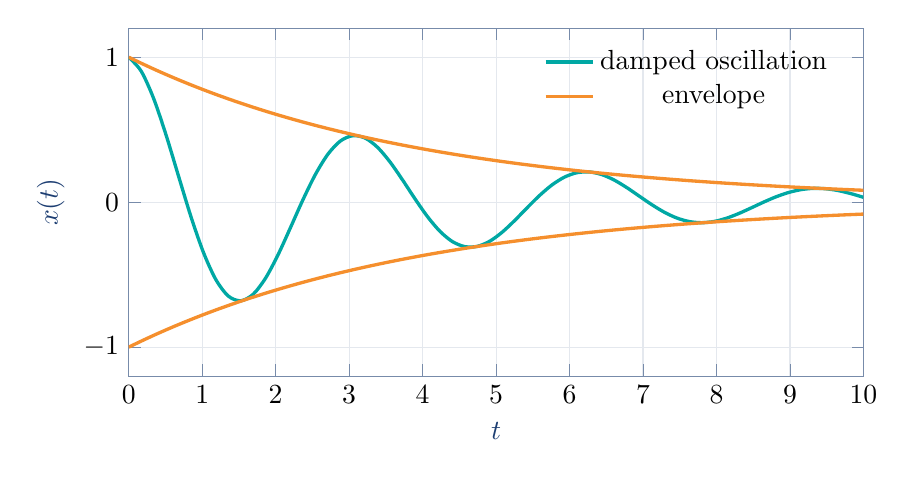
\begin{tikzpicture}
\begin{axis}[width=.9\textwidth, height=6cm, grid=major, xmin=0, xmax=10, domain=0:10, samples=60,
             xlabel={$t$}, ylabel={$x(t)$}, legend pos=north east]
  \addplot[very thick, tealx, smooth] {exp(-0.25*x)*cos(deg(2*x))};
  \addplot[very thick, accent, smooth] {exp(-0.25*x)};
  \addplot[very thick, accent, smooth, forget plot] {-exp(-0.25*x)};
  \legend{damped oscillation, envelope}
\end{axis}
\end{tikzpicture}
\end{center}

\begin{center}
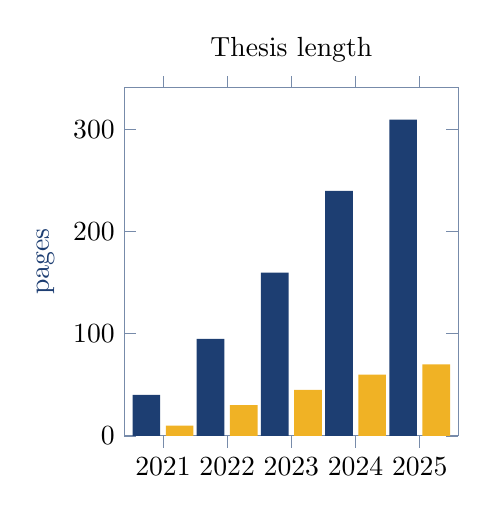
\begin{tikzpicture}
\begin{axis}[width=.48\textwidth, height=6cm, ybar, bar width=10pt, ymin=0, enlarge x limits=.15,
             symbolic x coords={2021,2022,2023,2024,2025}, xtick=data, ylabel={pages}, title={Thesis length}]
  \addplot[fill=navy, draw=none] coordinates {(2021,40) (2022,95) (2023,160) (2024,240) (2025,310)};
  \addplot[fill=gold, draw=none] coordinates {(2021,10) (2022,30) (2023,45) (2024,60) (2025,70)};
\end{axis}
\end{tikzpicture}\hfill
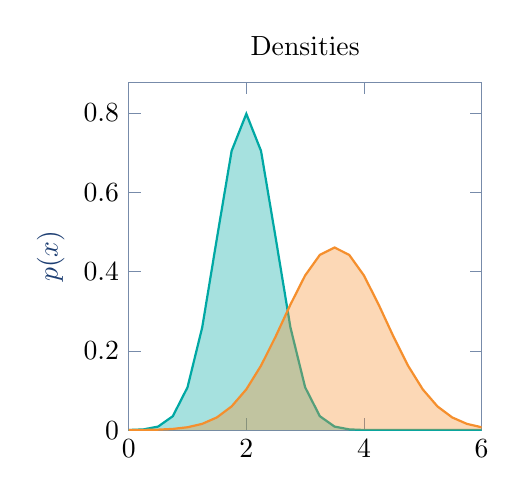
\begin{tikzpicture}
\begin{axis}[width=.5\textwidth, height=6cm, ymin=0, xmin=0, xmax=6, domain=0:6, samples=25, title={Densities}, ylabel={$p(x)$}, legend style={font=\small}]
  \addplot[draw=none, fill=tealx, fill opacity=.35] {exp(-(x-2)^2/0.5)/sqrt(0.5*pi)} \closedcycle;
  \addplot[thick, tealx] {exp(-(x-2)^2/0.5)/sqrt(0.5*pi)};
  \addplot[draw=none, fill=accent, fill opacity=.35] {exp(-(x-3.5)^2/1.5)/sqrt(1.5*pi)} \closedcycle;
  \addplot[thick, accent] {exp(-(x-3.5)^2/1.5)/sqrt(1.5*pi)};
\end{axis}
\end{tikzpicture}
\end{center}

\begin{center}
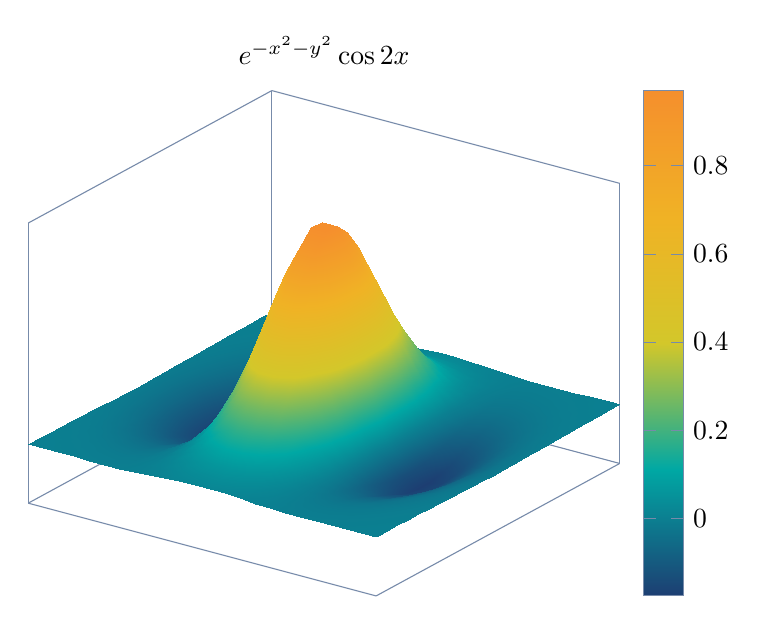
\begin{tikzpicture}
\begin{axis}[width=.75\textwidth, height=8cm, view={35}{30}, colormap={phi}{color=(navy) color=(tealx) color=(lime) color=(gold) color=(accent)},
             domain=-2:2, y domain=-2:2, samples=24, title={$e^{-x^2-y^2}\cos 2x$}, ticks=none, colorbar]
  \addplot3[surf, shader=interp] {exp(-x^2-y^2)*cos(deg(2*x))};
\end{axis}
\end{tikzpicture}
\end{center}

\end{document}
